\section{Durchführung}
\label{sec:durchfuehrung}

Der in diesem Versuch verwendete koaxiale Germaniumdetektor ist schematisch in \autoref{fig:aufbau} dargestellt.
\begin{figure}
    \centering
    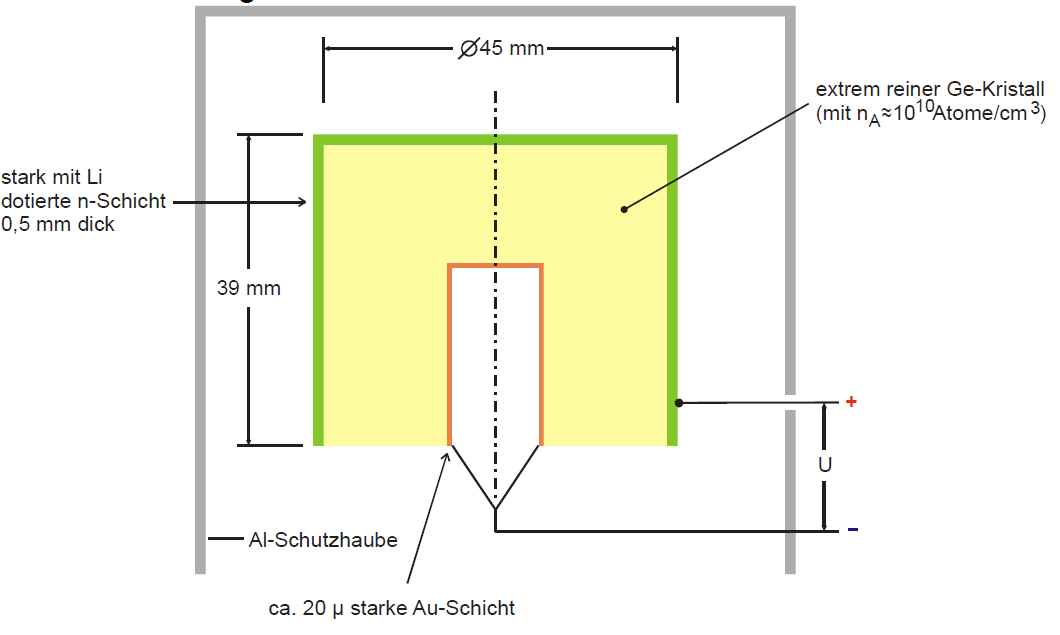
\includegraphics[width=\textwidth]{content/img/Abb_1.png}
    \caption{Schematische Darstellung eines koaxialen Germaniumdetektors \cite{versuchsanleitung}.
    Um eine Verarmungszone zu erzeugen,
    wurden die Außenseiten des Germanium-Kristalls jeweils p- und n-dotiert.
    Zusätzlich wird eine Spannung angelegt.}
    \label{fig:aufbau}
\end{figure}

Zur Erzeugung einer Verarmungszone wurden in die äußere Seite des Detektors Lithium-Atome eingearbeitet,
sodass diese n-dotiert ist.
Die innere Seite wurde durch Einfügen von Gold-Atomen p-dotiert.
Da die Dichte der freien positiven Ladungen in Germanium gering ist,
entsteht so eine asymmetrische Verarmungszone.
Um diese möglichst breit zu machen,
wird,
wie in \autoref{sec:funktionsweise} beschrieben,
eine äußere Spannung von \SI{5}{\kilo\volt} angelegt.
Der positive Pol ist dabei an die n-dotierte,
der negative an die p-dotierte Seite angeschlossen.
Zusätzlich ist der Detektor von einer Aluminiumschicht umgeben,
welche $\alpha$- und $\beta$- Strahlung aus den Zerfallsprozessen abschirmt.
Dies führt allerdings zu dazu,
dass die Energie der $\gamma$-Strahlung größer als \SI{150}{\kilo\eV} sein muss, um im Detektor nachgewiesen zu werden.
Zusätzlich wird der Detektor mithilfe von flüssigem Stickstoff gekühlt.
Die gemessenen Ströme werden mithilfe eines Stromverstärkers verstärkt und über einen Multichannel-Analyser ihrer Energie nach geordnet.

Zu Beginn der Messung wird die Energieauflösung und die Vollnachweiswahrscheinlichkeit des Detektors kalibiert,
indem das Spektrum von $\ce{^{152}Eu}$ ausgemessen wird.
Dazu wird eine entsprechende Quelle in einem gewissen Abstand zum Detektor befestigt,
um möglichst einen vollständigen Raumwinkel abzudecken.
Mithilfe eines Computerprogramms wird etwa \SI{45}{\minute} gemessen.
Anschließend wird die $\ce{^{152}Eu}$-Quelle durch eine $\ce{^{137}Cs}$-Quelle und anschließend durch eine $\ce{^{133}Ba}$-Quelle ersetzt,
deren Spektren über die gleiche Zeitdauer ausgemessen werden.
Danach wird ein Uran-Stein als unbekannte Quelle ohne räumlichen Abstand auf dem Detektor befestigt.
Dieses Spektrum wird über eine Dauer von etwa \SI{30}{\minute} gemessen.
Um den weiteren Untergrund zu bestimmen,
wird abschließend eine Messung ohne Probe gestartet,
%TODO: Zeitdauer erwähnen/Grund richtig? (Erinnerung an V01)
welche eine Dauer von etwa \SI{24}{\hour},
um möglichst viele Untergrundereignisse zu messen.